\documentclass[a4paper]{article}

\usepackage[utf8]{inputenc}
\usepackage{enumitem}
\usepackage{tikz}
\usepackage{amsmath}
\usepackage{amssymb}

\usepackage{anysize}

\usepackage{verbatim}


\marginsize{2.0cm}{2cm}{2.5cm}{2.5cm}

\author{Gruppe 6}

\title{\textbf{VerteilteWebInf Hausaufgabe 5}}
\date{\today}




\begin{document}
\maketitle


\section*{Aufgabe 1}
\begin{enumerate}[label=\alph*)]
\item \begin{verbatim}
SELECT v1.FlugNr as Flug1, v2.FlugNr as Flug2
FROM Flughaefen f1,Verbindungen v1, Verbindungen v2, Flughaefen f2
WHERE f1.Stadt='New-York' AND v1.von=f1.Code AND v1.nach=v2.von 
																	AND v2.nach=f2.Code AND f2.Stadt='Sydney'
				\end{verbatim}

\item Kanonische Übersetzung:

\tikzset{listingborder/.style={thick}}


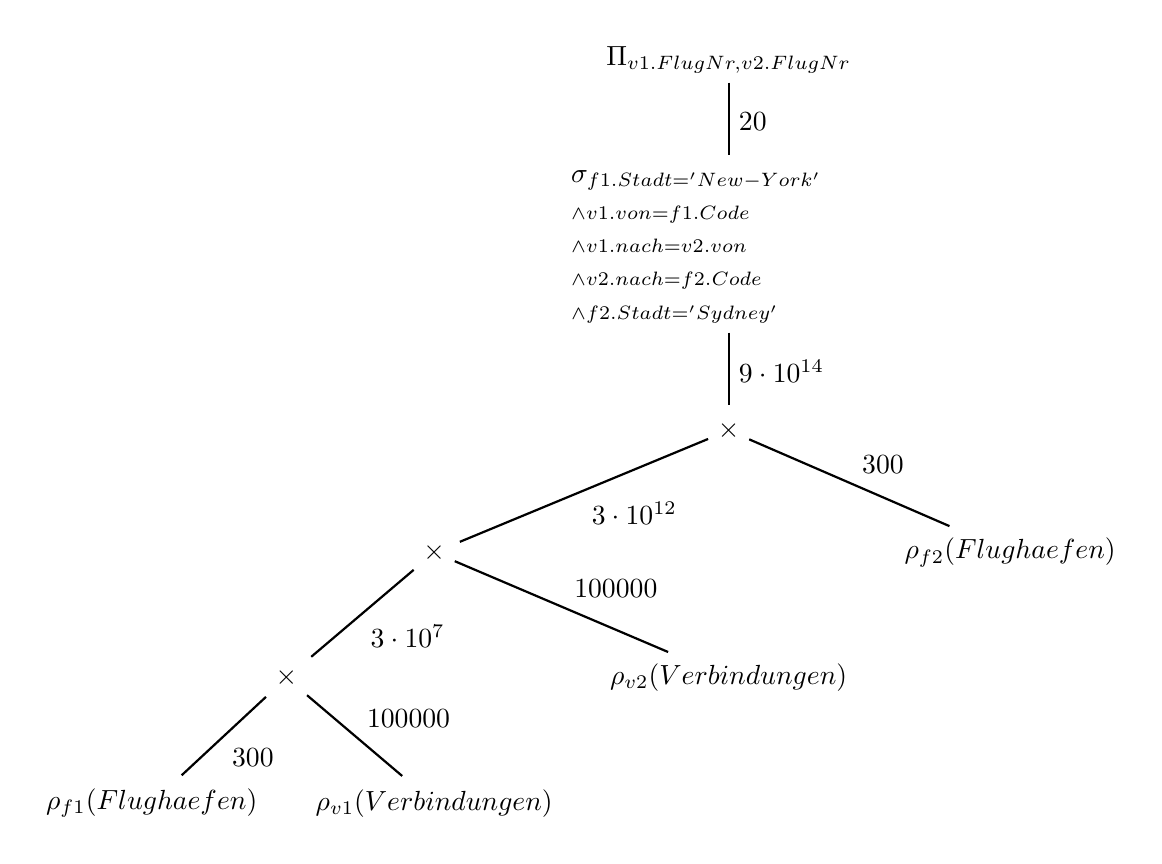
\begin{tikzpicture} [
    auto,
    block/.style    = { rectangle, draw=none,  text centered,
                        minimum height=5mm },
    line/.style     = { draw, thick, shorten >=2pt},
  ]


  % Define nodes in matrix
  \matrix [column sep=0mm, row sep=10mm] {
&&&&\node[block](project){$\Pi_{v1.FlugNr, v2.FlugNr}$}; \\
&&&&\node[block](select){\begin{minipage}{4cm}
$\sigma_{ f1.Stadt='New-York' }$ 
\newline $_{
\land v1.von=f1.Code}$ 
\newline $_{
\land v1.nach=v2.von}$
\newline $_{
\land v2.nach=f2.Code}$
\newline $_{
\land f2.Stadt='Sydney'}$
\end{minipage}};&&; \\
&&&&\node[block](times3){$\times$};&&\\
&&&\node[block](times2){$\times$};&&& \node[block](f2){$\rho_{f2}(Flughaefen)$};&; \\
&&\node[block](times1){$\times$};&&\node[block](v2){$\rho_{v2}(Verbindungen)$};& & \\
\node[block](f1){$\rho_{f1}(Flughaefen)$};&&&\node[block](v1){$\rho_{v1}(Verbindungen)$}; &&& \\
  };


  % connect the nodes
		\path [line] (times1) --node{300} (f1);
		\path [line] (times1) --node{100000} (v1);
		\path [line] (times2) --node{100000} (v2);
		\path [line] (times2) --node{$3\cdot 10^7$} (times1);
		\path [line] (times3) --node{300} (f2);
		\path [line] (times3) --node{$3\cdot 10^{12}$} (times2);
		\path [line] (select) --node{$9\cdot 10^{14}$} (times3);
		\path [line] (project) --node{20} (select);
\end{tikzpicture}\\
Die Zahlen an den Kanten geben die Größe der jeweiligen (Zwischen-) Relation an. Grundlage der Werte sind die Abschätzungen aus Teilaufgabe $c)$.

\item Relationsgrößen: 
$|Flughaefen|=300, |Verbindungen|=100.000$\\

Optimierter Baum:\\
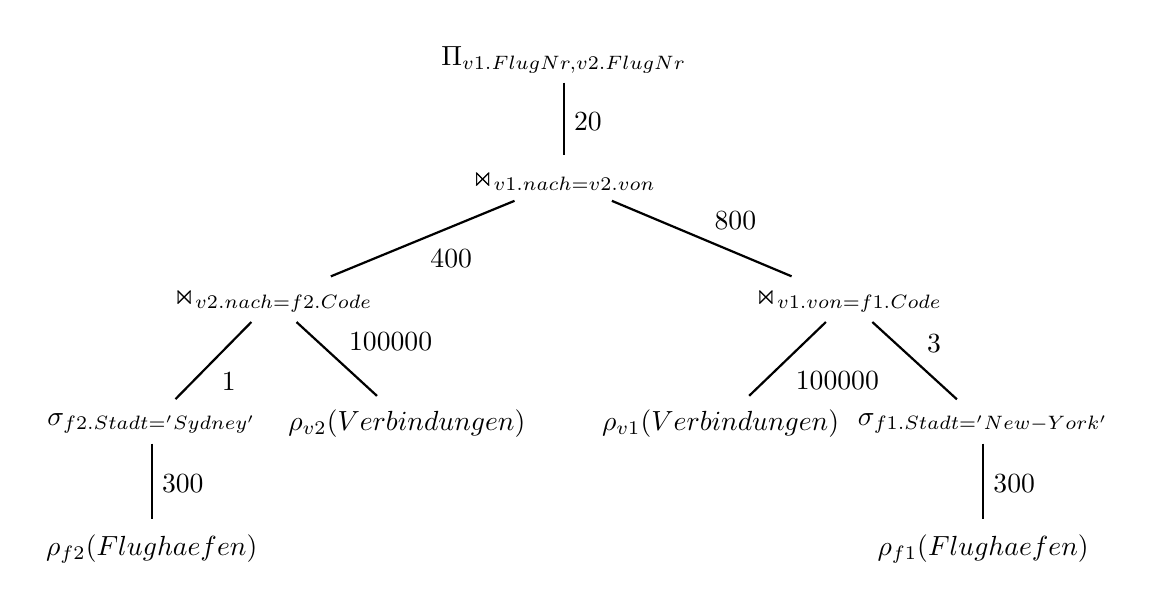
\begin{tikzpicture} [
    auto,
    block/.style    = { rectangle, draw=none,  text centered,
                        minimum height=5mm },
    line/.style     = { draw, thick, shorten >=2pt},
  ]


  % Define nodes in matrix
  \matrix [column sep=-13mm, row sep=10mm] {
&&&\node[block](project){$\Pi_{v1.FlugNr, v2.FlugNr}$}; \\
&&&\node[block](times3){$\Join_{v1.nach=v2.von}$}; \\
&\node[block](times1){$\Join_{v2.nach=f2.Code}$};&&&&\node[block](times2){$\Join_{v1.von=f1.Code}$};\\
\node[block](s2){$\sigma_{f2.Stadt='Sydney'}$};&&\node[block](v2){$\rho_{v2}(Verbindungen)$}; &&\node[block](v1){$\rho_{v1}(Verbindungen)$};&&\node [block](s1){$\sigma_{ f1.Stadt='New-York' }$}; \\
\node[block](f2){$\rho_{f2}(Flughaefen)$};&&&&&& \node[block](f1){$\rho_{f1}(Flughaefen)$}; \\
  };


  % connect the nodes
		\path [line] (times1) --node{1} (s2);
		\path [line] (s2) --node{300} (f2);
		\path [line] (times1) --node{100000} (v2);
		\path [line] (times2) --node{100000} (v1);
		\path [line] (times2) --node{3} (s1);
		\path [line] (times3) --node{400} (times1);
		\path [line] (times3) --node{800} (times2);
		\path [line] (s1) --node{300} (f1);
		\path [line] (project) --node{20} (times3);
\end{tikzpicture}\\

Dies stellt eine gravierende Verbesserung gegenüber der kanonischen Übersetzung dar, da kein Zwischenergebnis größer als 800 Tupel beinhaltet. Bei der kanonischen Übersetzung der SQL-Query beinhaltet die Zwischenrelation $9\cdot10^{14} $ Tupel, bevor die Selektion angewendet wird.

\item 

%%%%%%%%%%%%%%%%%%%%%%%%%%%%%%%%%%%%%%%
%%%%%%%%%%%%%%%%%%%%%%%%%%%%%%%%%%%%%%%
%
%
%
% Wie ist das mit den Gebieten gemeint? Zu welchem Gebiet gehören z.B. Transatlantikflüge?
%
%
%
%%%%%%%%%%%%%%%%%%%%%%%%%%%%%%%%%%%%%%%
%%%%%%%%%%%%%%%%%%%%%%%%%%%%%%%%%%%%%%%

Kanonischer Operatorbaum:\\
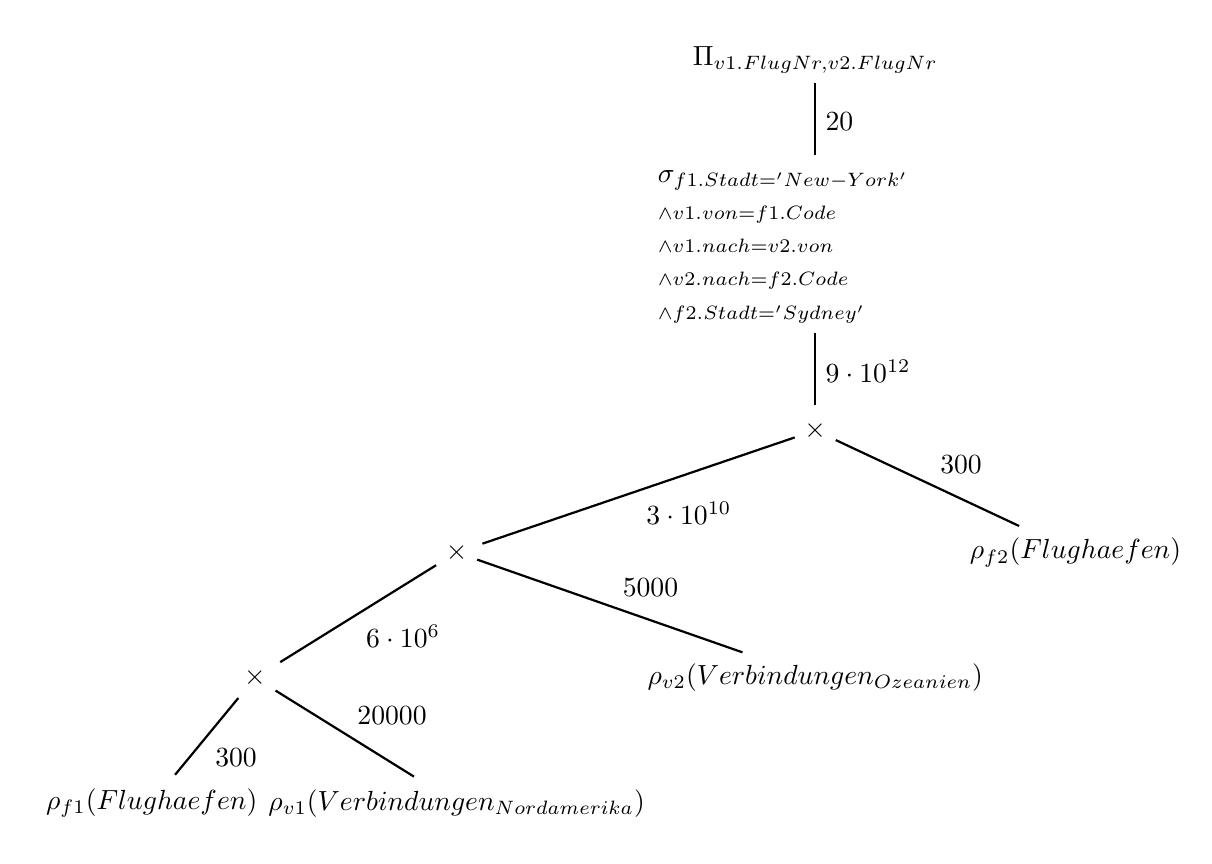
\begin{tikzpicture} [
    auto,
    block/.style    = { rectangle, draw=none,  text centered,
                        minimum height=5mm },
    line/.style     = { draw, thick, shorten >=2pt},
  ]


  % Define nodes in matrix
  \matrix [column sep=-2mm, row sep=10mm] {
&&&&\node[block](project){$\Pi_{v1.FlugNr, v2.FlugNr}$}; \\
&&&&\node[block](select){\begin{minipage}{4cm}
$\sigma_{ f1.Stadt='New-York' }$ 
\newline $_{
\land v1.von=f1.Code}$ 
\newline $_{
\land v1.nach=v2.von}$
\newline $_{
\land v2.nach=f2.Code}$
\newline $_{
\land f2.Stadt='Sydney'}$
\end{minipage}};&&; \\
&&&&\node[block](times3){$\times$};&&\\
&&&\node[block](times2){$\times$};&&& \node[block](f2){$\rho_{f2}(Flughaefen)$};&; \\
&&\node[block](times1){$\times$};&&\node[block](v2){$\rho_{v2}(Verbindungen_{Ozeanien})$};& & \\
\node[block](f1){$\rho_{f1}(Flughaefen)$};&&&\node[block](v1){$\rho_{v1}(Verbindungen_{Nordamerika})$}; &&& \\
  };


  % connect the nodes
		\path [line] (times1) --node{300} (f1);
		\path [line] (times1) --node{20000} (v1);
		\path [line] (times2) --node{5000} (v2);
		\path [line] (times2) --node{$6\cdot 10^6$} (times1);
		\path [line] (times3) --node{300} (f2);
		\path [line] (times3) --node{$3\cdot 10^{10}$} (times2);
		\path [line] (select) --node{$9\cdot 10^{12}$} (times3);
		\path [line] (project) --node{20} (select);
\end{tikzpicture}




Optimierter Baum:\\
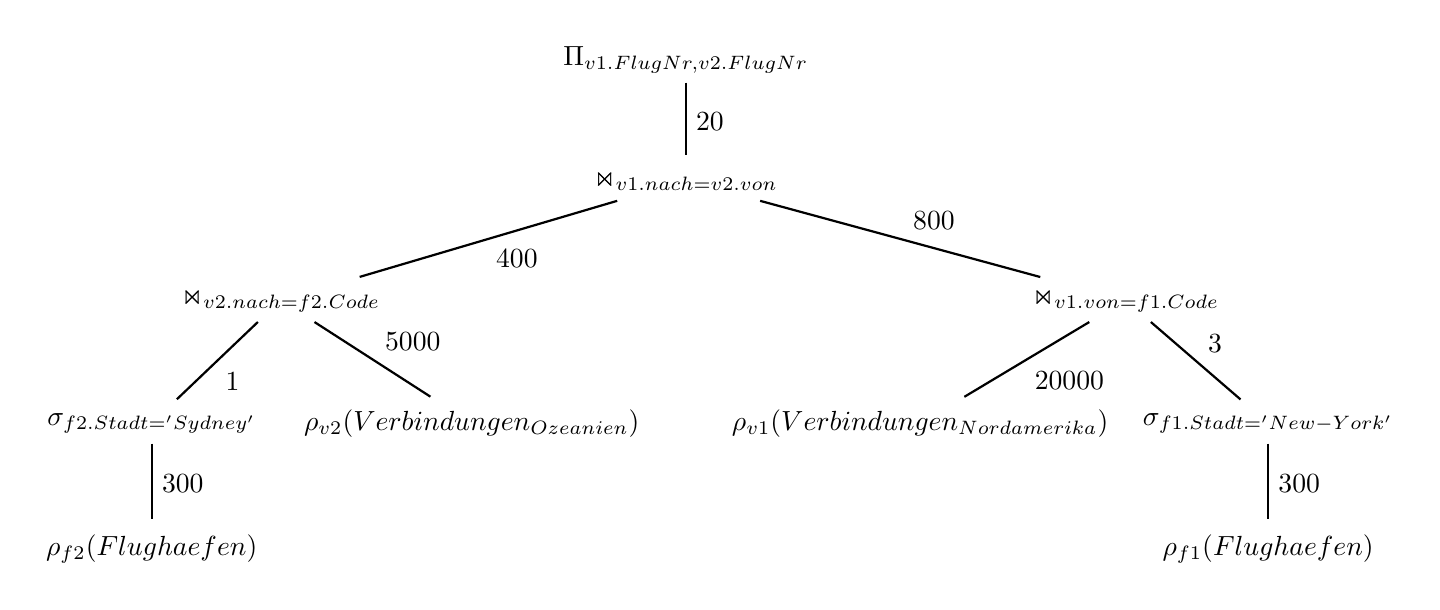
\begin{tikzpicture} [
    auto,
    block/.style    = { rectangle, draw=none,  text centered,
                        minimum height=5mm },
    line/.style     = { draw, thick, shorten >=2pt},
  ]


  % Define nodes in matrix
  \matrix [column sep=-12mm, row sep=10mm] {
&&&\node[block](project){$\Pi_{v1.FlugNr, v2.FlugNr}$}; \\
&&&\node[block](times3){$\Join_{v1.nach=v2.von}$}; \\
&\node[block](times1){$\Join_{v2.nach=f2.Code}$};&&&&\node[block](times2){$\Join_{v1.von=f1.Code}$};\\
\node[block](s2){$\sigma_{f2.Stadt='Sydney'}$};&&\node[block](v2){$\rho_{v2}(Verbindungen_{Ozeanien})$}; &&\node[block](v1){$\rho_{v1}(Verbindungen_{Nordamerika})$};&&\node [block](s1){$\sigma_{ f1.Stadt='New-York' }$}; \\
\node[block](f2){$\rho_{f2}(Flughaefen)$};&&&&&& \node[block](f1){$\rho_{f1}(Flughaefen)$}; \\
  };


  % connect the nodes
		\path [line] (times1) --node{1} (s2);
		\path [line] (s2) --node{300} (f2);
		\path [line] (times1) --node{5000} (v2);
		\path [line] (times2) --node{20000} (v1);
		\path [line] (times2) --node{3} (s1);
		\path [line] (times3) --node{400} (times1);
		\path [line] (times3) --node{800} (times2);
		\path [line] (s1) --node{300} (f1);
		\path [line] (project) --node{20} (times3);
\end{tikzpicture}
\end{enumerate}


\section*{Aufgabe 2}
\textbf{Messzeiten für kleinen Testdatensatz:}\\
----------------------------------------\\
Hash-Join\\
----------------------------------------\\
Zeit bis erstes Ergebnis: 659 ms\\
Zeit gesamt: 10421 ms\\
\\
----------------------------------------\\
X-Join\\
----------------------------------------\\
Zeit bis erstes Ergebnis: 321 ms\\
Zeit gesamt: 10099 ms\\
\\
----------------------------------------\\
NL-Join\\
----------------------------------------\\
Zeit bis erstes Ergebnis: 3921 ms\\
Zeit gesamt: 100052 ms\\
\\
\textbf{Messzeiten für gesamten Testdatensatz:}\\
TODO
\end{document}


